\documentclass[12pt]{article}

\title{The Anti-Global Warming Swindle}
\author{Maximillien Courchesne-Mackie (6168005) \\
             Patrick White (5936927)}
\date{\today}

\usepackage[left=2cm,right=2cm]{geometry}
\usepackage{graphicx}
\graphicspath{{./img/}}
\DeclareGraphicsExtensions{.pdf,.png,.jpg}
\setlength{\parindent}{0in}

\begin{document}
\maketitle
\newpage

\begin{abstract}
    Because global warming is a multi-national phenomenon which directly effect humans, the analysis of scientific evidence is vital. \textit{The Great Global Warming Swindle} is a documentary which masquerades as a scientific commentary on the state of global warming, but fails to provide credible or correct evidence to support it's claims. This report will identify and criticise the arguments fundamental to the view of the director using current peer-reviewed scientific knowledge and common sense.
\end{abstract}
\newpage

\tableofcontents
\newpage

\listoffigures
\listoftables
\newpage

\section*{Summary}
\newpage

\section{Introduction}
	Due to advances in various scientific fields concluding that there has been a significant rise in the Earth's temperature over the past century, the subject of global warming has become a household topic. Politicians have adopted the phenomenon as a major part of their campaign and some parties have made it the root of their platform. \\
	
	This unifying fact has given rise to groups of skeptics who reject the scientific consensus on climate change and put forth the idea that it is a political and economical campaign of fraud. Martin Durkin, the director of \textit{The Great Global Warming Swindle} is one of these skeptics. His film accuses the International Panel on Climate Change (IPCC) of being too political, asserts that man-made $CO_2$ is insignificant as a greenhouse gas and that the developed world is killing the African dream of sustainable development. \\
	
	This report will outline the major arguments Durkin proposes and will show how each of those arguments are either based on false data or poor interpretations of data. Our arguments will be representative of the current scientific consensus on the matter and will be complimented with proven and peer-reviewed data amassed through years of scientific study and analysis. The information will be conveyed in an accessible manner, allowing scientific lay-persons to follow our criticism of the documentary. \\

\section{Global Warming - An Overview}
	\textit{Global warming} is the increase of the temperature of Earth's climate and is usually studied over vast periods of time. The Earth's atmosphere retains a large portion of the heat emitted by the Sun thanks to a group of compounds known as \textit{greenhouse gases}. \textit{Human-caused global warming} is the increase of Carbon Dioxide ($CO_2$) in the atmosphere due to man-made systems which pollute the environment (non-electrical vehicles, mining, and factories for example). \\
	
	To fully understand the impact humans have on the global temperature, we need to understand the greenhouse effect. The greenhouse effect is what allows the Earth to remain heated by the Sun's rays and, without it, Earth would be inhabitable. It is due to a select number of compounds which are able to absorb and emit infrared radiation, called greenhouse gases. These gases form a protective shell around the Earth and absorb the Sun's radiation [...]. \\
	
\section{Arguments Presented}
    \textit{The Great Global Warming Swindle} does not provide any credible evidence to support their claims of a political and economic climate scandal, however the following section will extract the film's arguments and provide rebuttals that are founded in scientific fact.
    
\subsection{The Relevance of the Post Economic Boom}
    One of the fundamental arguments made by the film is that historic global climate data does not fit with the "theory" of global warming. They refer to a period roughly 25 years in length known as the \textit{World War II Post Economic Expansion} (or \textit{Postwar Economic Boom}). According to the film, temperatures should have risen during this period due to the increase in human activity, however the global climate data indicates a drop of temperature instead. Therefore, according to the makers of the film, global warming is a fraud and has been proven wrong in the past.\\
    
    Sadly, the film's interpretation of the climate data is seriously flawed. Below is a comparison the graph of the mean temperature change since 1880 (released by NASA) and the exact same graph as it appears in the documentary.
    
    \begin{figure}[h!]
        \centering
        \includegraphics[scale=0.3]{Instrumental_Temperature_Record.ps}
        \caption{Global Temperature Anomaly 1880-2010 (NASA, 2011)}
    \end{figure}
    
    \begin{figure}[h!]
        \centering
        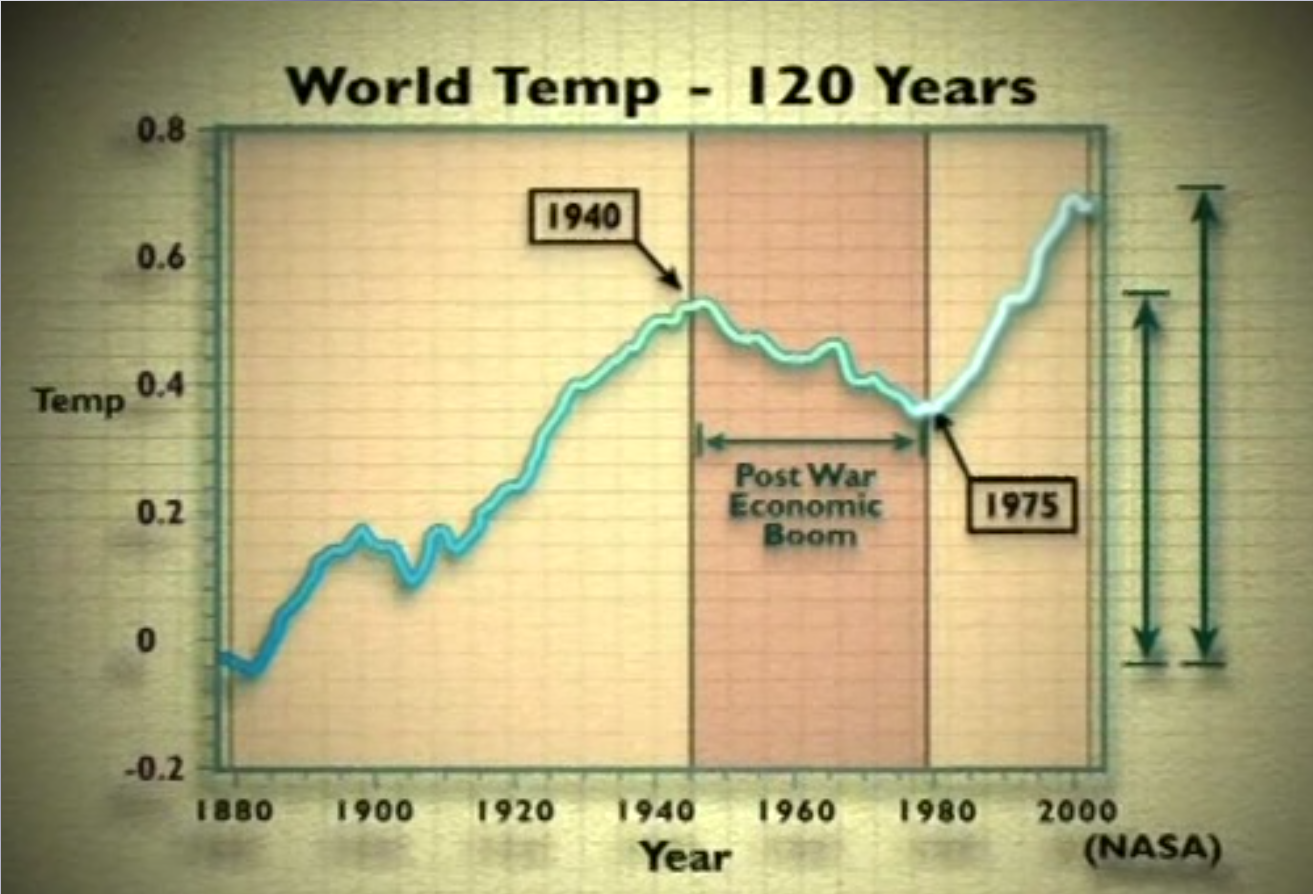
\includegraphics[scale=0.25]{fake_graph.ps}
        \caption{Global Temperature Anomaly as used by the film}
    \end{figure}
           
	- Film shows the graph\\
	- What was/is the post economic boom\\
	- How has the film interpreted the graph/data\\
	- What is the correct way of interpreting the data\\

\subsection{Global Warming is Politics}	
	
Another argument the film claims is how research in global warming has deviated from its original purpose and has become a political movement. The original goal behind the research was to look for scientific evidence of man made global warming. However, in today’s society it has become a political movement and accepted among society as a type of religion. Patrick Moore, the cofounder of Greenpeace, stated in the film that “if you do not believe in Global Warming, it’s is like you are a holocaust denier.” What the film failed to mention, that was discussed earlier in the report, was the scientific data they used was not real data but manipulated in order to show that global warming is not caused by humans. This is the reason behind society not accepting their scientific claims.\\  

Additionally, Professor Paul Reiter, a former member of the International Panel for Climate Change (IPCC), we he resigned from his involved the IPCC still included his name in their report on malaria. However, Professor Martin Parry who was the co-chair for the IPCC assessment report stated in an email: “Dr. Reiter was not selected … it would have been impossible for him to resign.” With this statement, it is clear that Dr. Reiter was not even selected to be on the board of scientist and that is not why his name was on the report. Martin Parry then stated “ Dr. Reiter was invited to be an IPCC reviewer, and we did in fact get review comments from Paul.” Therefore, he was named a reviewer for the report and his claims were in correct.\\

\subsection{The Sun Drives Elevated Tempurature}

Dr. Piers Corbyn, a Climate Forecaster, introduced the argument that the solar activity is the driving factor of global warming. The main argument is how the study of sunspots has a correlation with the temperature on earth. He presented the following graph of the temperature and solar activity over the past 400 years. The blue line, left y-axis, graphs the temperature and the red line, right y-axis, graphs the solar activity.   \\

% Need to insert the diagram here\\

The trends seen on the graph have some similarities, however when analysing the past 20 years the solar activity should shoot up which I does not. Also, between 1700 and 1800, there is a significant increase in solar activity and according to Dr. Corbyn there should have also been a significant increase of earth temperatures yet there is not. \\

Furthermore, the producers of the film have tampered with the graph in order to create this “trend.” The following statement is from Friss-Christensen, the original publicers of the graph, “We have concerns regarding the use of a graph featured in the documentary titled ‘Temp and Solar Activity 400 Years’. Firstly, we have reason to believe that parts of the graph were made up of fabricated data that were presented as genuine. The inclusion of the artificial data is both misleading and pointless.” Therefore, any statement in regard to this topic is fraud and it’s conclusion that solar activity drives climate change is in conclusion and should be disregarded by viewers of the film. \\

Finally, the following diagram is from a study from the Stanford Solar Center. Their research topic was Solar Variability and Global Warming. In the graph the red line represents the temperature, blue is $CO_2$ levels, and the gold line is the sunspot number also referred to solar activity. \\

% Need to insert the diagram here

The trends for this graph have some similar patterns until the 20\textsuperscript {<th>} century. The argument discussed in section \textit{The Relevance of the Post Economic Boom} was the decrease in temperature through the economic boom when human $CO_2$ were high, but in the graph above it is clear that the number of sun spots in increase from 1930 to 1960 at a steady rate which demonstrate a contradiction in Dr. Piers Corbyn statement. In addition, the end of the 20\textsuperscript {<th>} century and beginning of the 21\textsuperscript {<th>} century there is an increase in both the temperature and the $CO_2$ level but there is a decreasing levels of sunspot showing another contradiction. Therefore, the argument made the producers of the film does not fit with real external scientific data.  \\


\subsection{The Insignificance of $CO_2$}

In the opening scene of the documentary, Professor Ian Clark, department of Earth Science at the University of Ottawa states that “We can not say that $C0_2$ will drive climate, it certainly never did in the past.” It is clear that the film is trying to show that $C0_2$ is an insignificant factor in the current climate charges. The following two graph, which show the relationship between $CO_2$ and historical temperate, provides evidence that there is a direct relationship between the amount of $CO_2$ in the atmosphere and temperature. On the first graph the red line is the measurement of temperature and the blue lines graphs the amount of $CO_2$ in the atmosphere. The second graph is from analysing ice cores, the blue line represents the levels of $CO_2$ and the black line is the levels of deuterium, a hydrogen isotope, which represents the historical temperature.\\

% Need to insert the diagram here\\

In analysing the above graphs, the historical levels of $CO_2$ in the atmosphere follows a very similar trends as the temperature. This is yet another scientific records that falsifies the statements made by the scientist in this documentary. Furthermore, referring to “Figure #. 3.3” from the 1950’s to the present there is a consistent in temperature, the red curve, also there is an increase is the amount of $CO_2$ in the atmosphere, this is another justification for the effects of $CO_2$ on temperature. \\

Another argument that the documents attempts to prove is that the amount of $CO_2$ produced by humans in insignificant compared to other sources. There is a short cartoon clip in the film showing that volcanoes emitting $CO_2$ with the narrator stating “Volcanoes produce more $CO_2$ each year that all the factories and cars and planes and other sources of man-made carbon dioxide put together.” This fact is fictitious and complete irrelevant to the main argument that $CO_2$ is not the leading cause of climate change. The following is a statement by the USGS, an organization that studies the effects of Volcanoes, in reference to Volcanic Gases and Their Effects, “Human activities release more that 130 times the amount of $CO_2$ emitted by volcanoes.” This is scientific research proving that the statement made by the narrator was simply fabricated and false. \\

\section{Solution Presented}
	- Film says funding for global warming research should be ceased\\
	- Also that people should stop caring and doing things to stop it\\
	- Simply wrong, based on the facts. The solution doesn't stand up\\
	- Best course of action is to keep researching in the global warming field and to work together to create a cleaner society.\\
\section{Conclusion}
	- The film fails to provide concrete evidence to support their claims and solutions\\
	- The science seems to have been altered to provide seemingly convincing evidence to those not versed in the global warming field \\
	- A piece of propaganda \\
\section{References}
235

\end{document}